% CVPR 2022 Paper Template
% based on the CVPR template provided by Ming-Ming Cheng (https://github.com/MCG-NKU/CVPR_Template)
% modified and extended by Stefan Roth (stefan.roth@NOSPAMtu-darmstadt.de)

\documentclass[10pt,onecolumn,letterpaper]{article}

%%%%%%%%% PAPER TYPE  - PLEASE UPDATE FOR FINAL VERSION
% \usepackage[review]{cvpr}      % To produce the REVIEW version
\usepackage{cvpr}              % To produce the CAMERA-READY version
%\usepackage[pagenumbers]{cvpr} % To force page numbers, e.g. for an arXiv version

% Include other packages here, before hyperref.
\usepackage{graphicx}
\usepackage{amsmath}
\usepackage{amssymb}
\usepackage{booktabs}
\usepackage{csquotes}
\usepackage{caption}
\usepackage{subcaption}

% It is strongly recommended to use hyperref, especially for the review version.
% hyperref with option pagebackref eases the reviewers' job.
% Please disable hyperref *only* if you encounter grave issues, e.g. with the
% file validation for the camera-ready version.
%
% If you comment hyperref and then uncomment it, you should delete
% ReviewTempalte.aux before re-running LaTeX.
% (Or just hit 'q' on the first LaTeX run, let it finish, and you
%  should be clear).
\usepackage[pagebackref,breaklinks,colorlinks]{hyperref}


% Support for easy cross-referencing
\usepackage[capitalize]{cleveref}
\crefname{section}{Sec.}{Secs.}
\Crefname{section}{Section}{Sections}
\Crefname{table}{Table}{Tables}
\crefname{table}{Tab.}{Tabs.}


%%%%%%%%% PAPER ID  - PLEASE UPDATE
\def\cvprPaperID{*****} % This is obsolete
\def\confName{CVPR}
\def\confYear{2022}


\begin{document}

%%%%%%%%% TITLE
\title{Warmstarting with fidelities}

\author{Janis Fix, Leon Gieringer, Furkan Kara\\
{\small \{fixj, gieringl, karaf\}@cs.uni-freiburg.de}
% For a paper whose authors are all at the same institution,
% omit the following lines up until the closing ``}''.
% Additional authors and addresses can be added with ``\and'',
% just like the second author.
% To save space, use either the email address or home page, not both
}
\maketitle

%%%%%%%%% ABSTRACT
%\begin{abstract}
%    We implemented a framework to warmstart a hyperparameter optimization (HPO) algorithm with different fidelities.
%\end{abstract}

%%%%%%%%% BODY TEXT
\section{Introduction}
\label{sec:intro}
Hyperparameter optimization is computationally very expensive which is why many speedup techniques were developed.
Especially multi-fidelity improved its performance, e.g. by focussing on promissing configurations (Hyperband) \cite{Li2016} or by intelligently sampling interesting configurations using bayesian optimization \cite{Falkner2018}.
In order to find the most promissing configurations, we need to train them and evaluate their performance for every fidelity.
However the current implementations of those algorithms train by discarding the achieved progress from the last fidelity and start from scratch every time.
There is research about saving such interim results and continuing later on, but its focussed merely on the fidelity epochs (Freeze-Thaw) \cite{Swersky2014}.
Our goal was to use this approach for the fidelity subsets.
Furthermore we wanted to create a framework to use different fidelities to learn insights about the training behaviour.

%Research Questions from neeratyoy:
%\begin{itemize}
%    \item Do we need one or more fidelities and checkpointing?
%    \item How do we allow for continuation for fidelities?
%    \item What can we learn about the optimisation?
%\end{itemize}
%What is the main goal we want to achieve? is it performance, efficiency, ...?
%Since some research was already performed in this topic (regarding warmstarting), what do we try to do differently?
%We tried to generate a experimenting framework to enable warmstarting with different fidelities.
%Hereby we allow to run the experiments with separate fidelities as well as them joined together.
%The purpose behind this approach was to gain insides of the training behaviour as well as the influence of different fidelity-mixes.
%Also interesting for us was to see the amount of influence each fidelity has for the training - and thus the hyperparameter configuration choices.\\

%How did we approach it? selected fidelities,


\section{Methodology}

\section{Results}
\begin{figure}[h]
    \centering
    \begin{subfigure}[b]{0.24\textwidth}
        \centering
        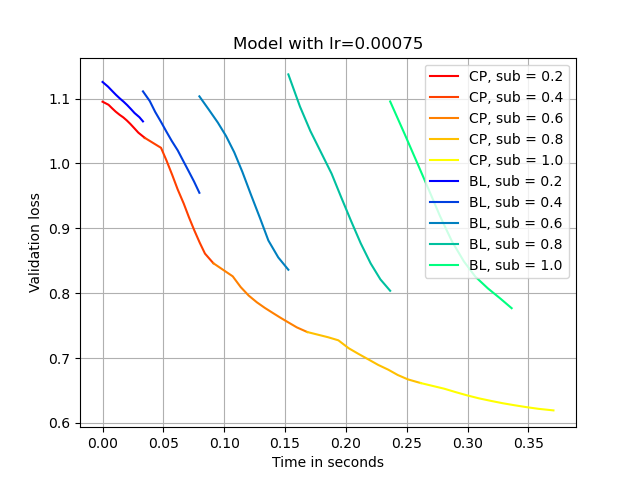
\includegraphics[width=\textwidth]{figures/22_07/iris/loss_time_0.00075.png}
        \caption{IRIS}
        \label{fig:13a}
    \end{subfigure}
    %\hfill
    \begin{subfigure}[b]{0.24\textwidth}
        \centering
        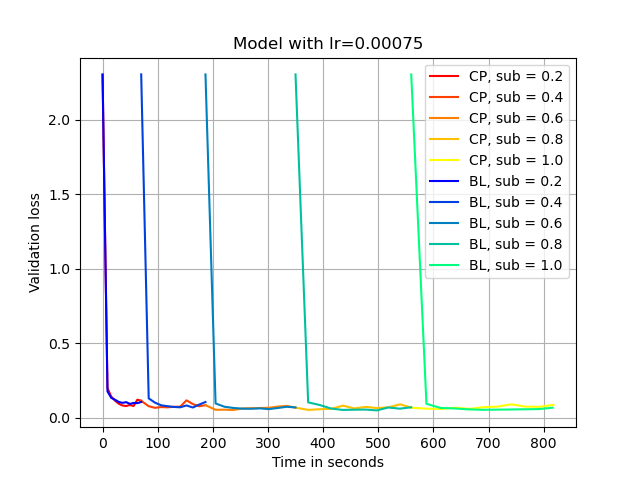
\includegraphics[width=\textwidth]{figures/22_07/10ep/loss_time_0.00075.png}
        \caption{MNIST 10 epochs}
        \label{fig:13b}
    \end{subfigure}
    %\hfill
    \begin{subfigure}[b]{0.24\textwidth}
        \centering
        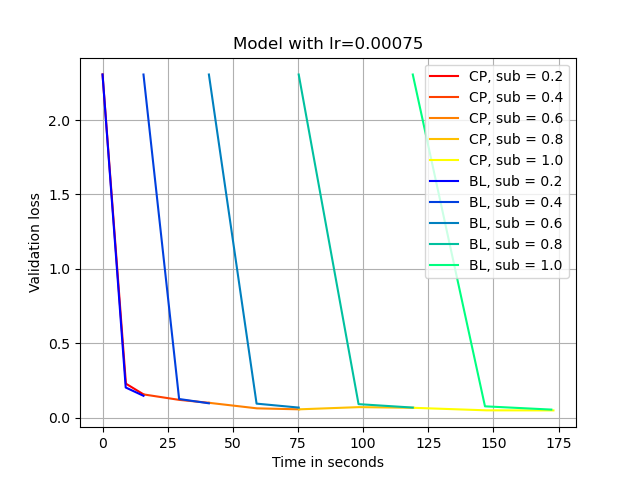
\includegraphics[width=\textwidth]{figures/22_07/2ep/loss_time_0.00075.png}
        \caption{MNIST 2 epochs}
        \label{fig:13c}
    \end{subfigure}
    %\hfill
    \begin{subfigure}[b]{0.24\textwidth}
        \centering
        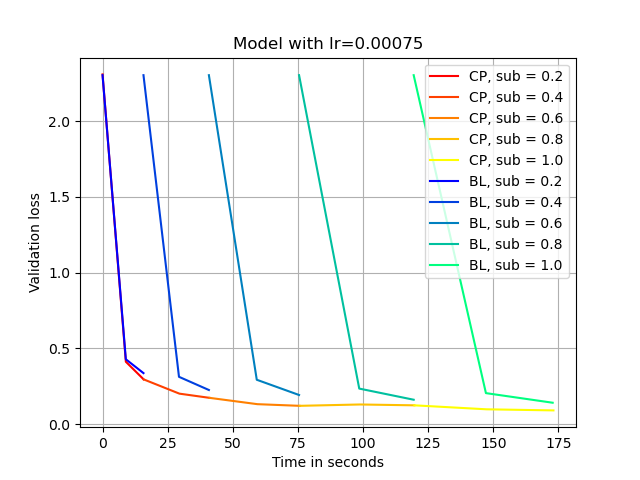
\includegraphics[width=\textwidth]{figures/22_07/2ep_smaller/loss_time_0.00075.png}
        \caption{MNIST 2 epochs, small model}
        \label{fig:13d}
    \end{subfigure}
    \caption{Visualization of validation loss versus training time for Adam optimizer and learning rate $7.5e^{-4}$}
    \label{fig:three graphs}
\end{figure}

\begin{figure}[h]
    \centering
    \begin{subfigure}[b]{0.24\textwidth}
        \centering
        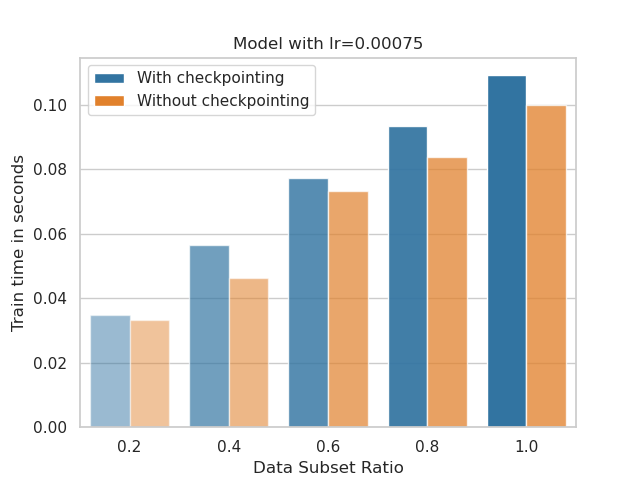
\includegraphics[width=\textwidth]{figures/22_07/iris/train_subset_0.00075.png}
        \caption{IRIS}
        \label{fig:19a}
    \end{subfigure}
    %\hfill
    \begin{subfigure}[b]{0.24\textwidth}
        \centering
        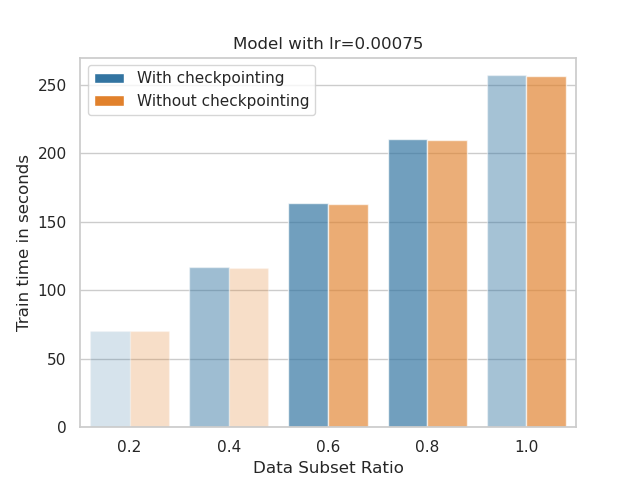
\includegraphics[width=\textwidth]{figures/22_07/10ep/train_subset_0.00075.png}
        \caption{MNIST 10 epochs}
        \label{fig:19b}
    \end{subfigure}
    %\hfill
    \begin{subfigure}[b]{0.24\textwidth}
        \centering
        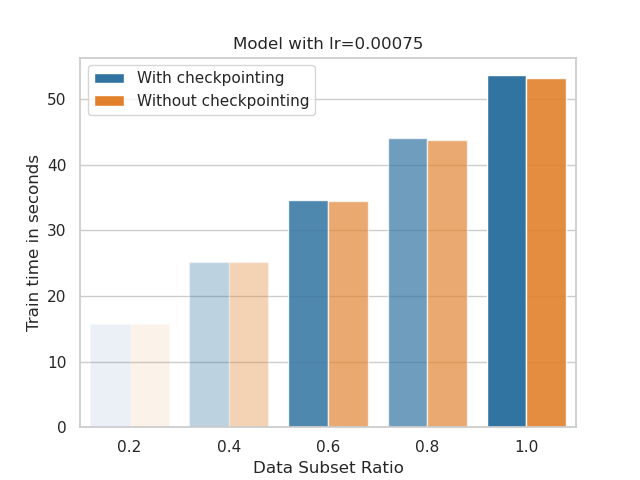
\includegraphics[width=\textwidth]{figures/22_07/2ep/train_subset_0.00075.png}
        \caption{MNIST 2 epochs}
        \label{fig:19c}
    \end{subfigure}
    %\hfill
    \begin{subfigure}[b]{0.24\textwidth}
        \centering
        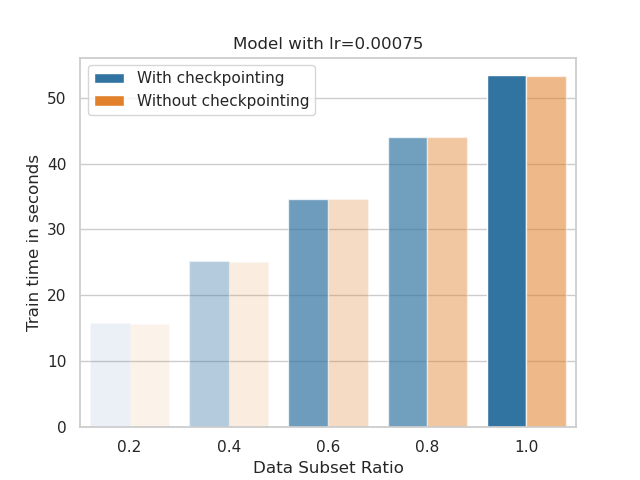
\includegraphics[width=\textwidth]{figures/22_07/2ep_smaller/train_subset_0.00075.png}
        \caption{MNIST 2 epochs, small model}
        \label{fig:19d}
    \end{subfigure}
    \caption{Visualization of the training time for every data subset ratio. A higher opacity means small validation performance difference to the optimum. An Adam optimizer and learning rate $7.5e^{-4}$ were used}
    \label{fig:19}
\end{figure}

\clearpage
\section{Summary}

%%%%%%%%% REFERENCES
{\small
\bibliographystyle{ieee_fullname}
\bibliography{egbib}
}
%%%%%%%%% APPENDIX
\clearpage
\appendix
\section{Graphs}
\subsection{Validation Loss}
\begin{figure}[h]
    \centering
    \begin{subfigure}[b]{0.24\textwidth}
        \centering
        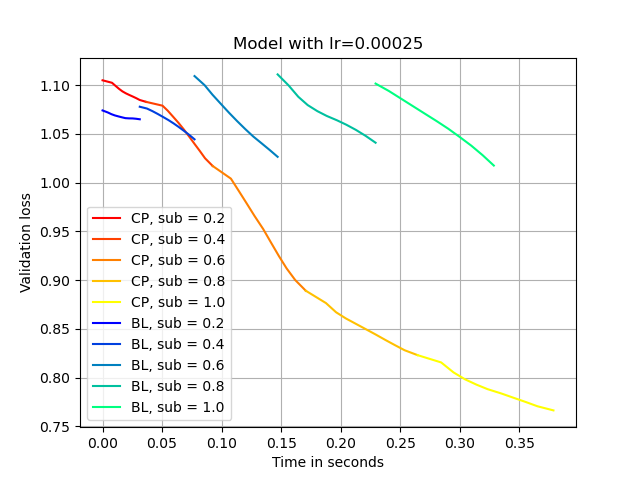
\includegraphics[width=\textwidth]{figures/22_07/iris/loss_time_0.00025.png}
        \caption{IRIS}
        \label{fig:1a}
    \end{subfigure}
    %\hfill
    \begin{subfigure}[b]{0.24\textwidth}
        \centering
        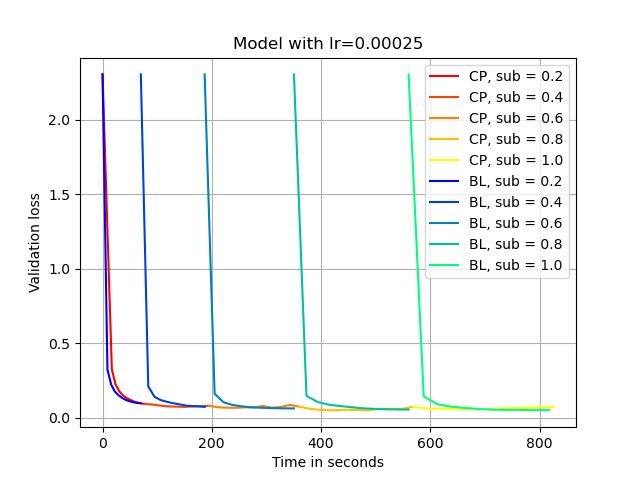
\includegraphics[width=\textwidth]{figures/22_07/10ep/loss_time_0.00025.png}
        \caption{MNIST 10 epochs}
        \label{fig:1b}
    \end{subfigure}
    %\hfill
    \begin{subfigure}[b]{0.24\textwidth}
        \centering
        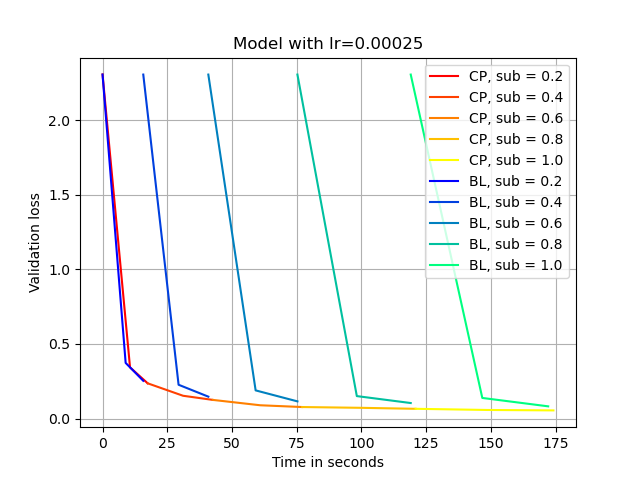
\includegraphics[width=\textwidth]{figures/22_07/2ep/loss_time_0.00025.png}
        \caption{MNIST 2 epochs}
        \label{fig:1c}
    \end{subfigure}
    %\hfill
    \begin{subfigure}[b]{0.24\textwidth}
        \centering
        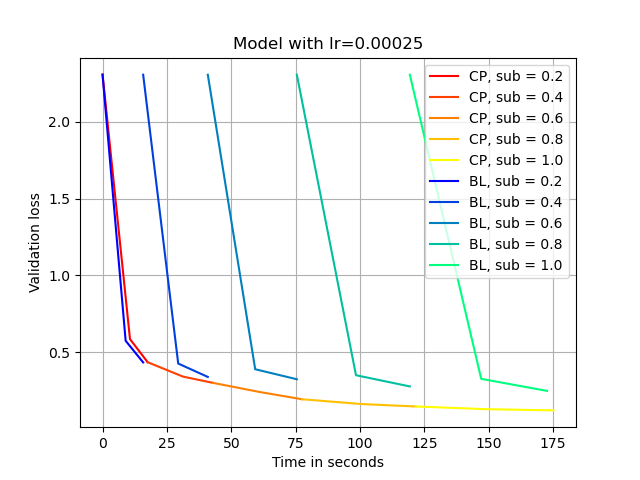
\includegraphics[width=\textwidth]{figures/22_07/2ep_smaller/loss_time_0.00025.png}
        \caption{MNIST 2 epochs, small model}
        \label{fig:1d}
    \end{subfigure}
    \caption{Visualization of validation loss versus training time for Adam optimizer and learning rate $2.5e^{-4}$}
    \label{fig:three graphs}
\end{figure}


\begin{figure}[h]
    \centering
    \begin{subfigure}[b]{0.24\textwidth}
        \centering
        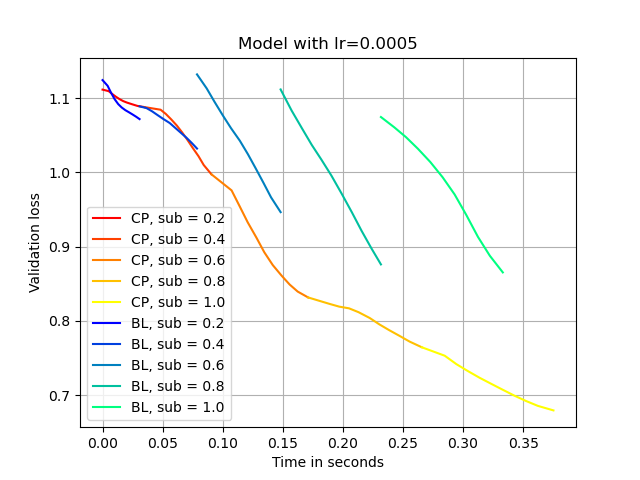
\includegraphics[width=\textwidth]{figures/22_07/iris/loss_time_0.0005.png}
        \caption{IRIS}
        \label{fig:2a}
    \end{subfigure}
    %\hfill
    \begin{subfigure}[b]{0.24\textwidth}
        \centering
        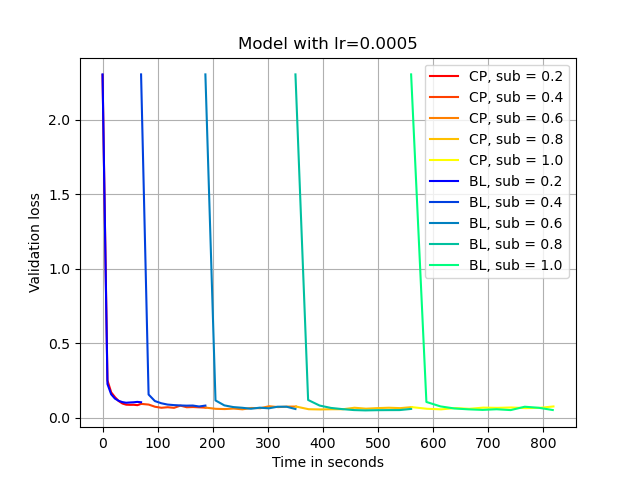
\includegraphics[width=\textwidth]{figures/22_07/10ep/loss_time_0.0005.png}
        \caption{MNIST 10 epochs}
        \label{fig:2b}
    \end{subfigure}
    %\hfill
    \begin{subfigure}[b]{0.24\textwidth}
        \centering
        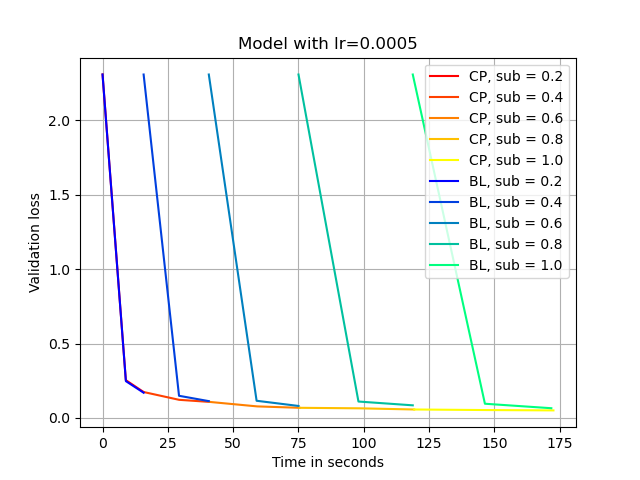
\includegraphics[width=\textwidth]{figures/22_07/2ep/loss_time_0.0005.png}
        \caption{MNIST 2 epochs}
        \label{fig:2c}
    \end{subfigure}
    %\hfill
    \begin{subfigure}[b]{0.24\textwidth}
        \centering
        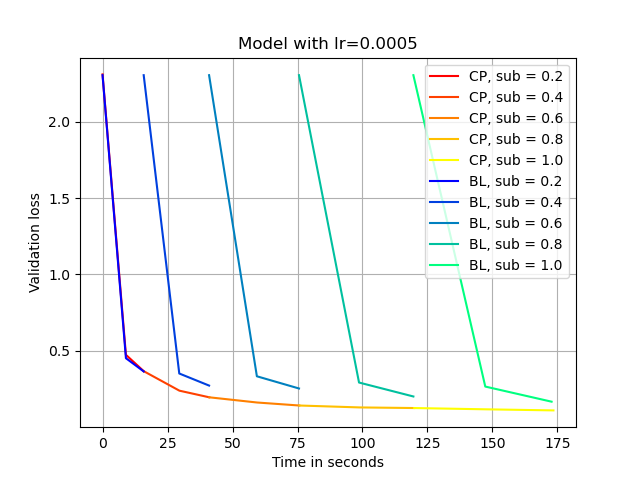
\includegraphics[width=\textwidth]{figures/22_07/2ep_smaller/loss_time_0.0005.png}
        \caption{MNIST 2 epochs, small model}
        \label{fig:2d}
    \end{subfigure}
    \caption{Visualization of validation loss versus training time for Adam optimizer and learning rate $5e^{-4}$}
    \label{fig:three graphs}
\end{figure}


\begin{figure}[h]
    \centering
    \begin{subfigure}[b]{0.24\textwidth}
        \centering
        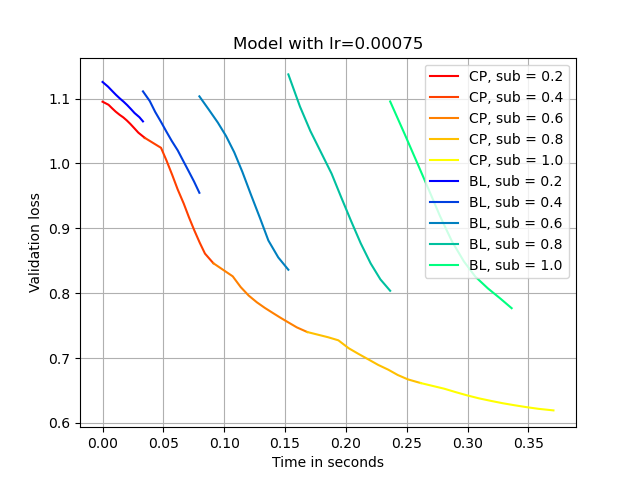
\includegraphics[width=\textwidth]{figures/22_07/iris/loss_time_0.00075.png}
        \caption{IRIS}
        \label{fig:3a}
    \end{subfigure}
    %\hfill
    \begin{subfigure}[b]{0.24\textwidth}
        \centering
        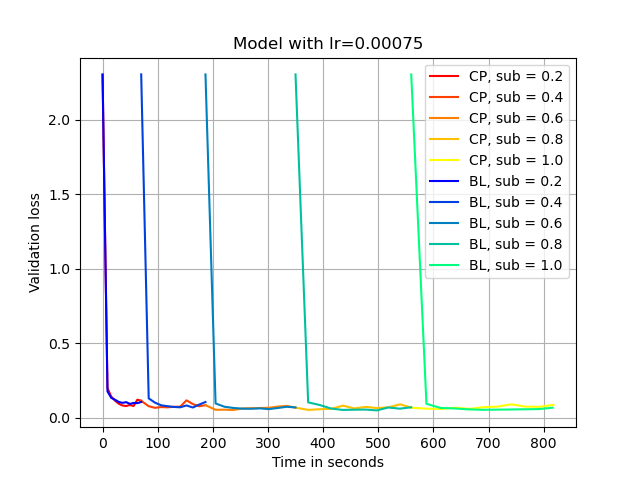
\includegraphics[width=\textwidth]{figures/22_07/10ep/loss_time_0.00075.png}
        \caption{MNIST 10 epochs}
        \label{fig:3b}
    \end{subfigure}
    %\hfill
    \begin{subfigure}[b]{0.24\textwidth}
        \centering
        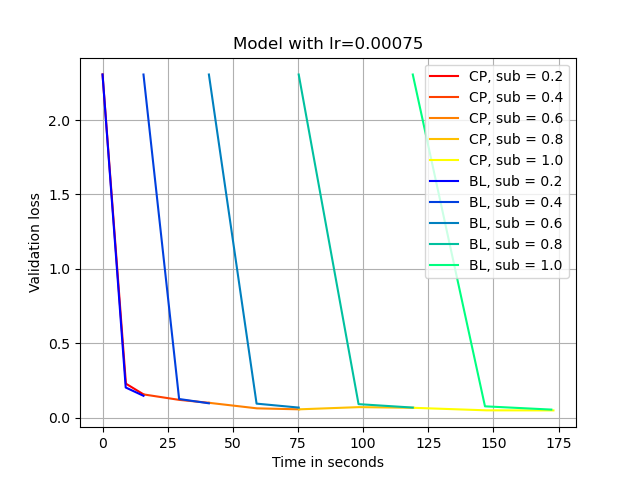
\includegraphics[width=\textwidth]{figures/22_07/2ep/loss_time_0.00075.png}
        \caption{MNIST 2 epochs}
        \label{fig:3c}
    \end{subfigure}
    %\hfill
    \begin{subfigure}[b]{0.24\textwidth}
        \centering
        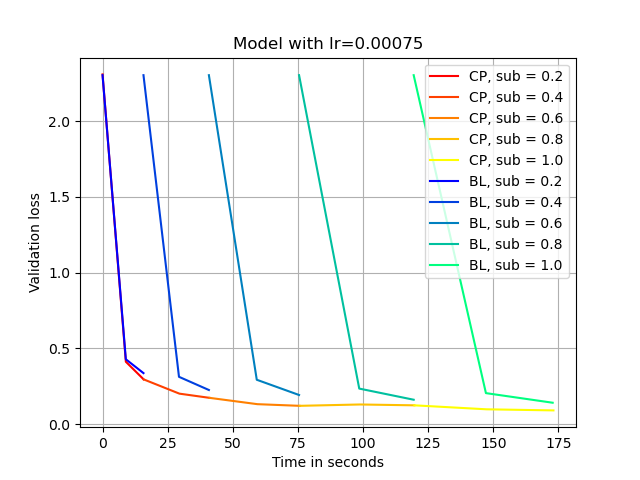
\includegraphics[width=\textwidth]{figures/22_07/2ep_smaller/loss_time_0.00075.png}
        \caption{MNIST 2 epochs, small model}
        \label{fig:3d}
    \end{subfigure}
    \caption{Visualization of validation loss versus training time for Adam optimizer and learning rate $7.5e^{-4}$}
    \label{fig:three graphs}
\end{figure}

\begin{figure}[h]
    \centering
    \begin{subfigure}[b]{0.24\textwidth}
        \centering
        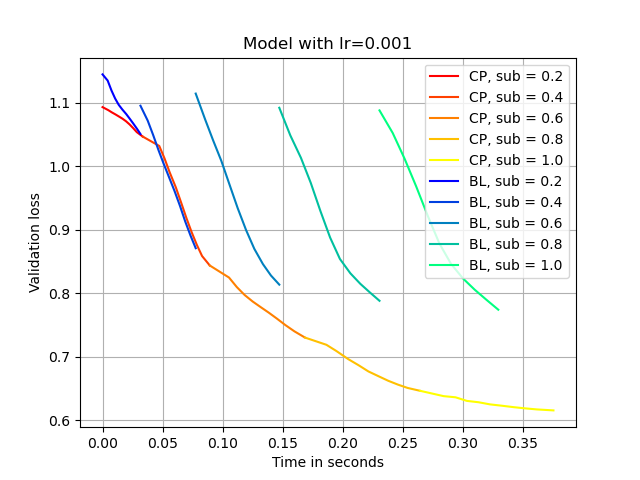
\includegraphics[width=\textwidth]{figures/22_07/iris/loss_time_0.001.png}
        \caption{IRIS}
        \label{fig:4a}
    \end{subfigure}
    %\hfill
    \begin{subfigure}[b]{0.24\textwidth}
        \centering
        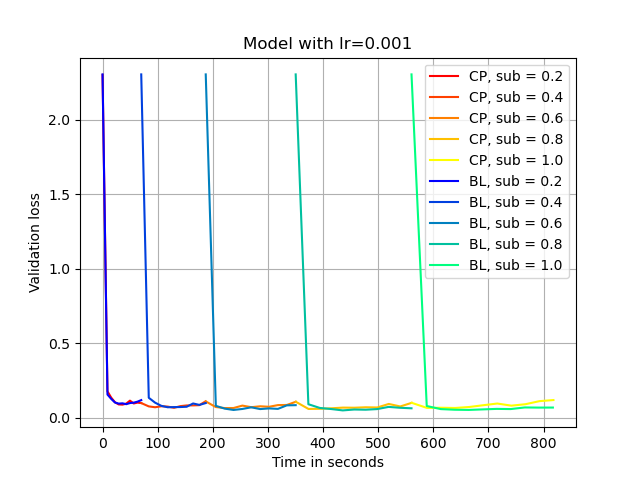
\includegraphics[width=\textwidth]{figures/22_07/10ep/loss_time_0.001.png}
        \caption{MNIST 10 epochs}
        \label{fig:4b}
    \end{subfigure}
    %\hfill
    \begin{subfigure}[b]{0.24\textwidth}
        \centering
        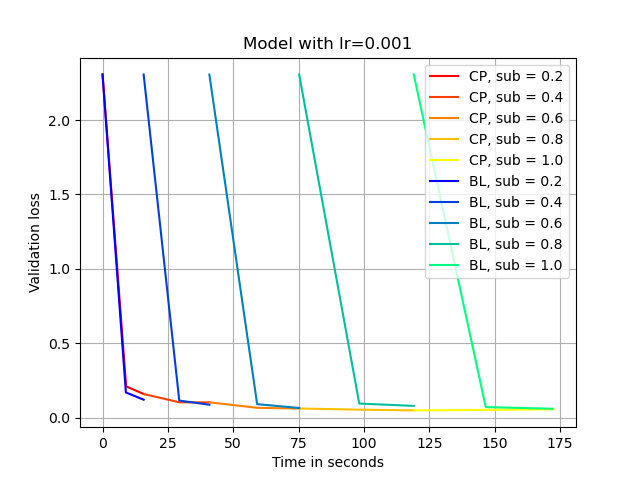
\includegraphics[width=\textwidth]{figures/22_07/2ep/loss_time_0.001.png}
        \caption{MNIST 2 epochs}
        \label{fig:4c}
    \end{subfigure}
    %\hfill
    \begin{subfigure}[b]{0.24\textwidth}
        \centering
        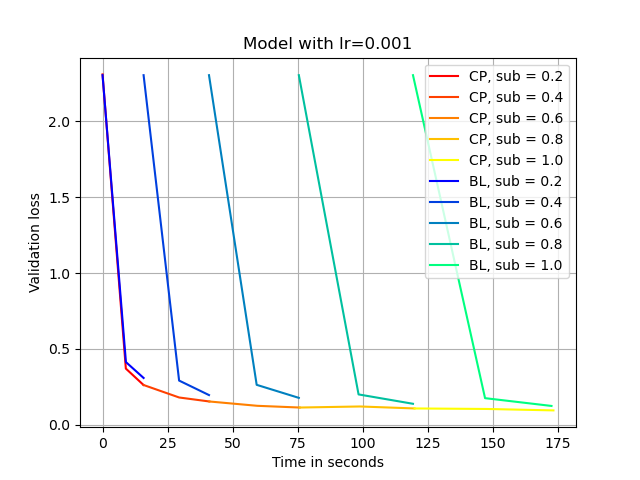
\includegraphics[width=\textwidth]{figures/22_07/2ep_smaller/loss_time_0.001.png}
        \caption{MNIST 2 epochs, small model}
        \label{fig:4d}
    \end{subfigure}
    \caption{Visualization of validation loss versus training time for Adam optimizer and learning rate $1e^{-3}$}
    \label{fig:three graphs}
\end{figure}


\begin{figure}[h]
    \centering
    \begin{subfigure}[b]{0.24\textwidth}
        \centering
        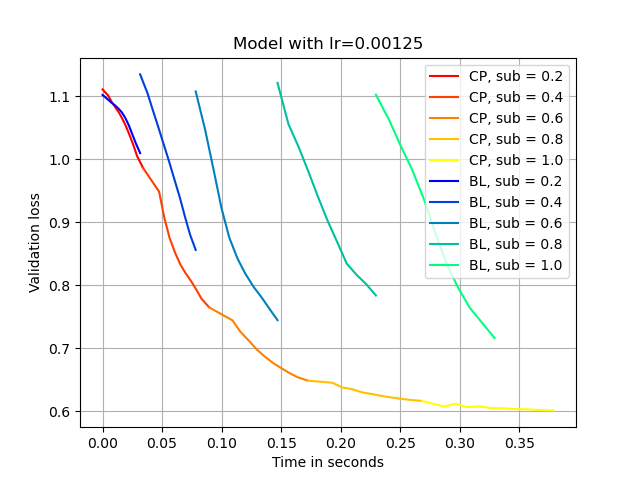
\includegraphics[width=\textwidth]{figures/22_07/iris/loss_time_0.00125.png}
        \caption{IRIS}
        \label{fig:5a}
    \end{subfigure}
    %\hfill
    \begin{subfigure}[b]{0.24\textwidth}
        \centering
        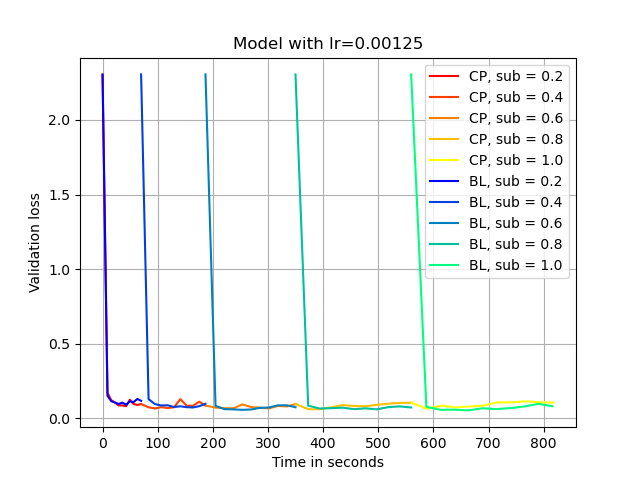
\includegraphics[width=\textwidth]{figures/22_07/10ep/loss_time_0.00125.png}
        \caption{MNIST 10 epochs}
        \label{fig:5b}
    \end{subfigure}
    %\hfill
    \begin{subfigure}[b]{0.24\textwidth}
        \centering
        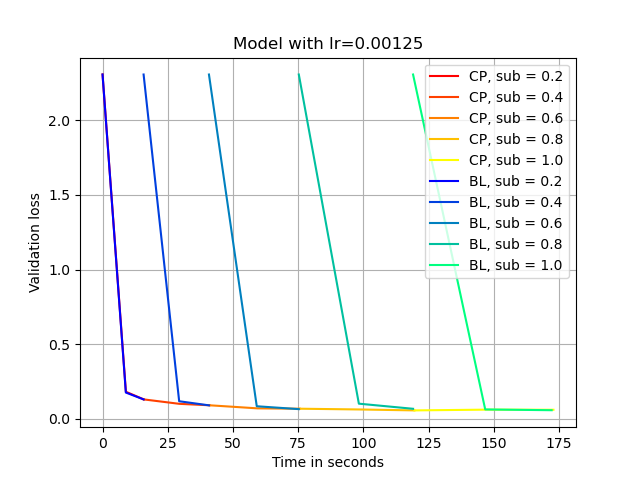
\includegraphics[width=\textwidth]{figures/22_07/2ep/loss_time_0.00125.png}
        \caption{MNIST 2 epochs}
        \label{fig:5c}
    \end{subfigure}
    %\hfill
    \begin{subfigure}[b]{0.24\textwidth}
        \centering
        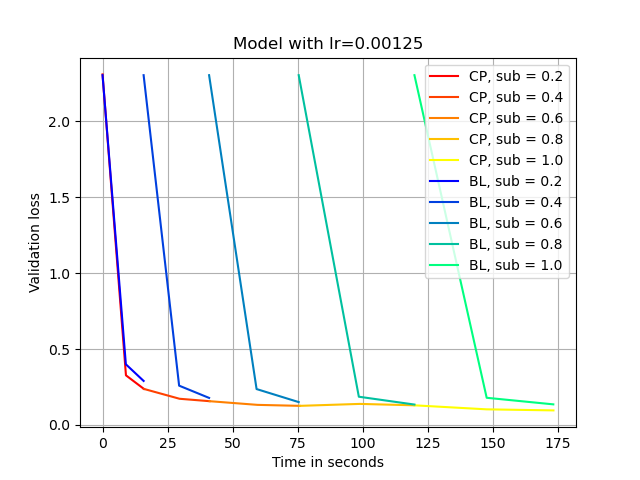
\includegraphics[width=\textwidth]{figures/22_07/2ep_smaller/loss_time_0.00125.png}
        \caption{MNIST 2 epochs, small model}
        \label{fig:5d}
    \end{subfigure}
    \caption{Visualization of validation loss versus training time for Adam optimizer and learning rate $1.25e^{-3}$}
    \label{fig:three graphs}
\end{figure}


\newpage
\subsection{Train Time}

\begin{figure}[h]
    \centering
    \begin{subfigure}[b]{0.24\textwidth}
        \centering
        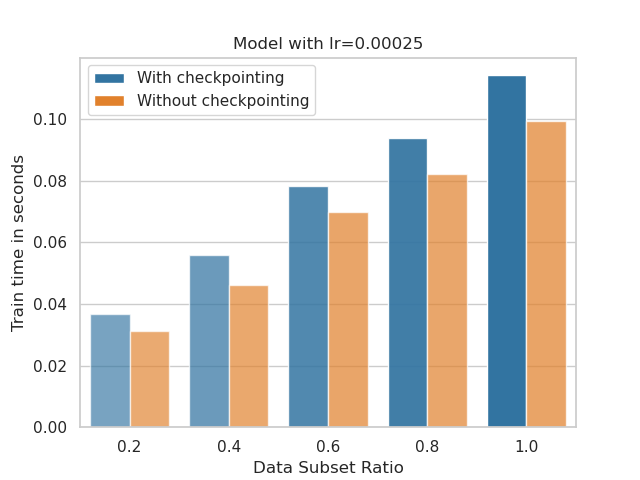
\includegraphics[width=\textwidth]{figures/22_07/iris/train_subset_0.00025.png}
        \caption{IRIS}
        \label{fig:7a}
    \end{subfigure}
    %\hfill
    \begin{subfigure}[b]{0.24\textwidth}
        \centering
        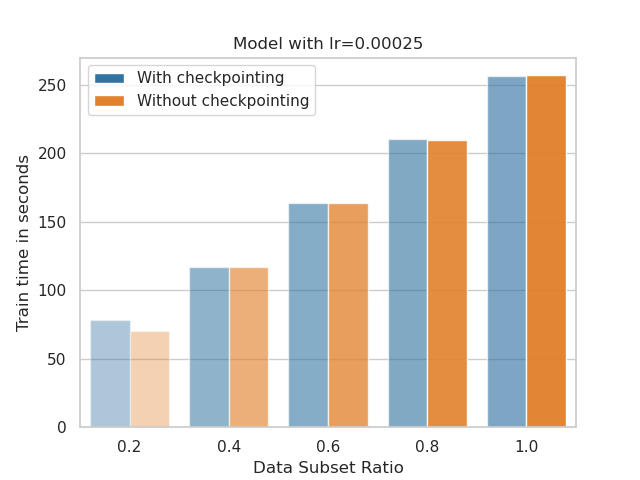
\includegraphics[width=\textwidth]{figures/22_07/10ep/train_subset_0.00025.png}
        \caption{MNIST 10 epochs}
        \label{fig:7b}
    \end{subfigure}
    %\hfill
    \begin{subfigure}[b]{0.24\textwidth}
        \centering
        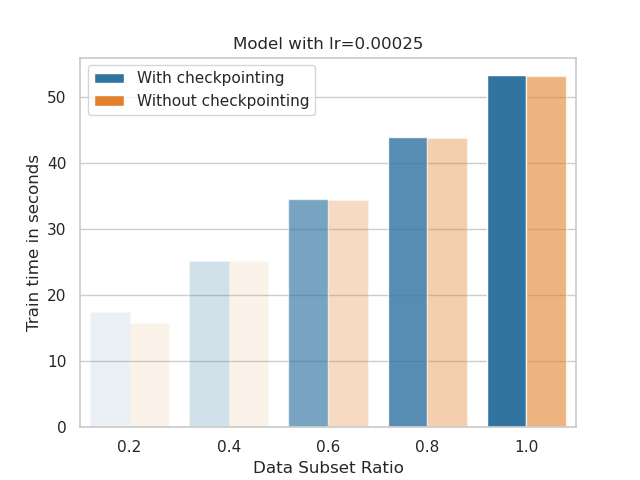
\includegraphics[width=\textwidth]{figures/22_07/2ep/train_subset_0.00025.png}
        \caption{MNIST 2 epochs}
        \label{fig:7c}
    \end{subfigure}
    %\hfill
    \begin{subfigure}[b]{0.24\textwidth}
        \centering
        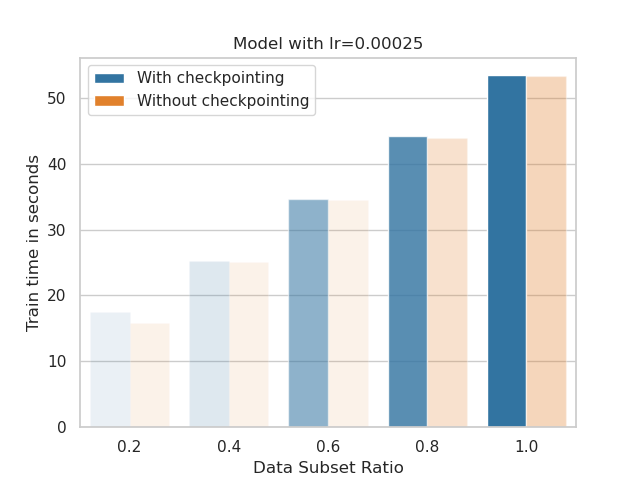
\includegraphics[width=\textwidth]{figures/22_07/2ep_smaller/train_subset_0.00025.png}
        \caption{MNIST 2 epochs, small model}
        \label{fig:7d}
    \end{subfigure}
    \caption{Visualization of the training time for every data subset ratio. A higher opacity means small validation performance difference to the optimum. An Adam optimizer and learning rate $2.5e^{-4}$ were used}
    \label{fig:7}
\end{figure}

\begin{figure}[h]
    \centering
    \begin{subfigure}[b]{0.24\textwidth}
        \centering
        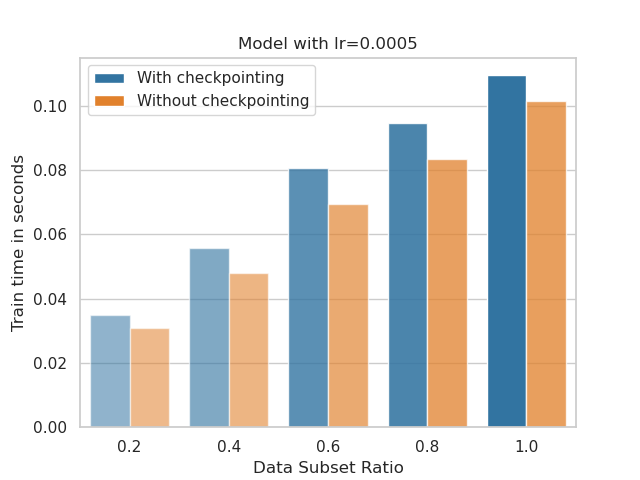
\includegraphics[width=\textwidth]{figures/22_07/iris/train_subset_0.0005.png}
        \caption{IRIS}
        \label{fig:8a}
    \end{subfigure}
    %\hfill
    \begin{subfigure}[b]{0.24\textwidth}
        \centering
        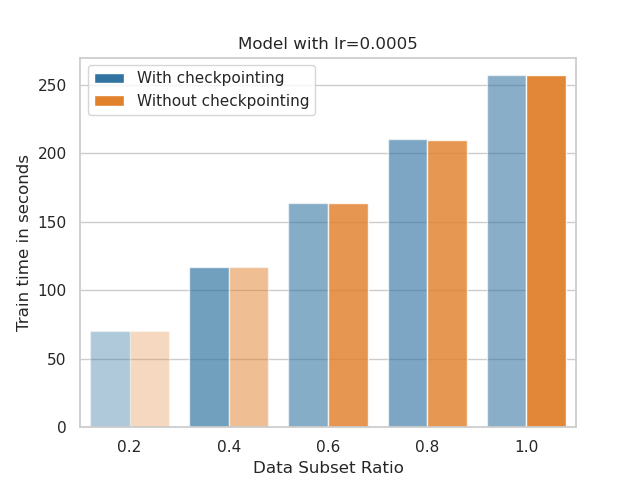
\includegraphics[width=\textwidth]{figures/22_07/10ep/train_subset_0.0005.png}
        \caption{MNIST 10 epochs}
        \label{fig:8b}
    \end{subfigure}
    %\hfill
    \begin{subfigure}[b]{0.24\textwidth}
        \centering
        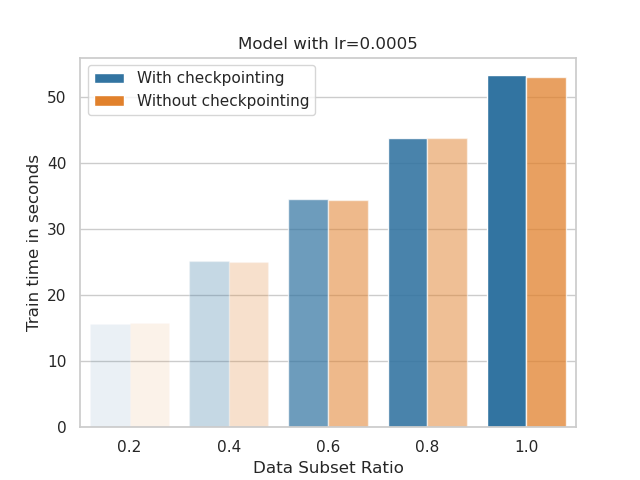
\includegraphics[width=\textwidth]{figures/22_07/2ep/train_subset_0.0005.png}
        \caption{MNIST 2 epochs}
        \label{fig:8c}
    \end{subfigure}
    %\hfill
    \begin{subfigure}[b]{0.24\textwidth}
        \centering
        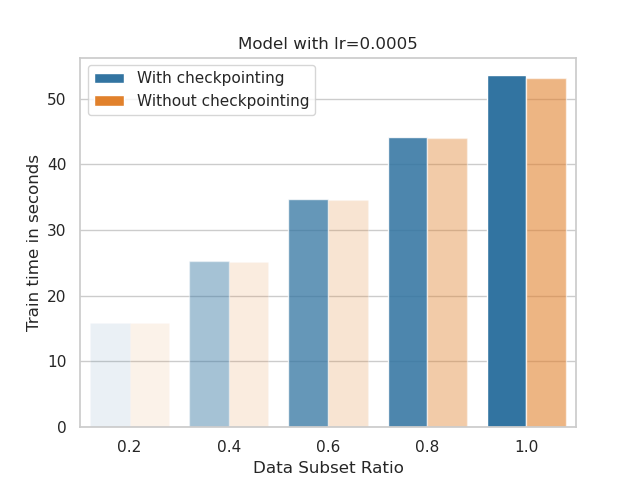
\includegraphics[width=\textwidth]{figures/22_07/2ep_smaller/train_subset_0.0005.png}
        \caption{MNIST 2 epochs, small model}
        \label{fig:8d}
    \end{subfigure}
    \caption{Visualization of the training time for every data subset ratio. A higher opacity means small validation performance difference to the optimum. An Adam optimizer and learning rate $5e^{-4}$ were used}
    \label{fig:8}
\end{figure}

\begin{figure}[h]
    \centering
    \begin{subfigure}[b]{0.24\textwidth}
        \centering
        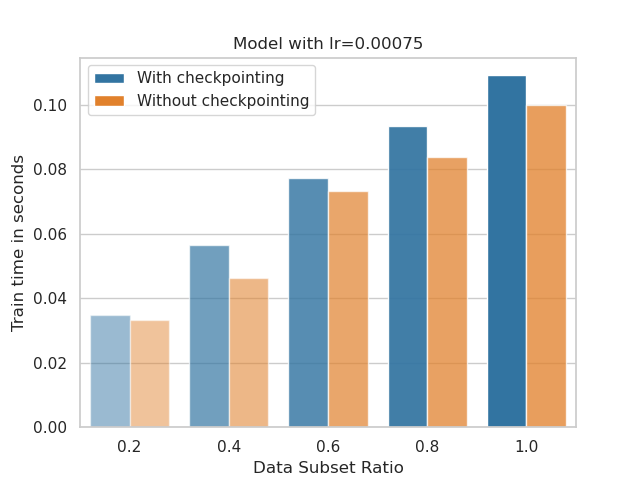
\includegraphics[width=\textwidth]{figures/22_07/iris/train_subset_0.00075.png}
        \caption{IRIS}
        \label{fig:9a}
    \end{subfigure}
    %\hfill
    \begin{subfigure}[b]{0.24\textwidth}
        \centering
        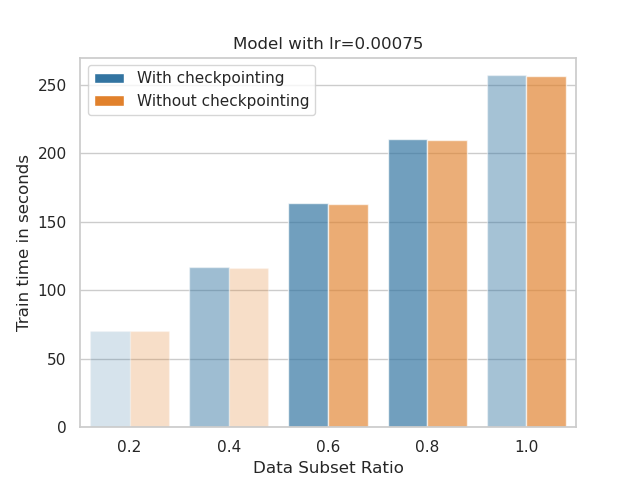
\includegraphics[width=\textwidth]{figures/22_07/10ep/train_subset_0.00075.png}
        \caption{MNIST 10 epochs}
        \label{fig:9b}
    \end{subfigure}
    %\hfill
    \begin{subfigure}[b]{0.24\textwidth}
        \centering
        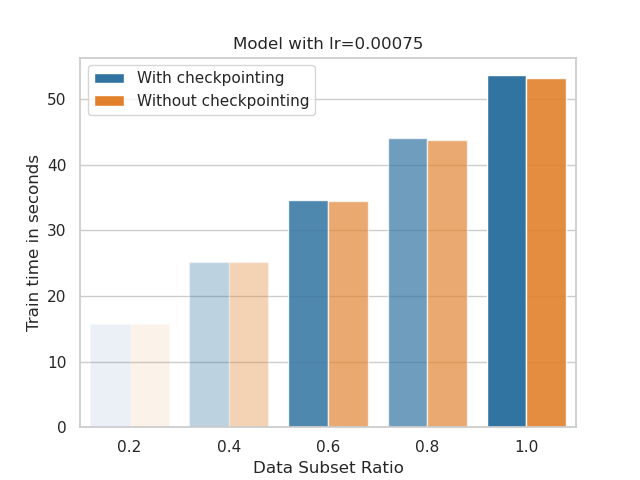
\includegraphics[width=\textwidth]{figures/22_07/2ep/train_subset_0.00075.png}
        \caption{MNIST 2 epochs}
        \label{fig:9c}
    \end{subfigure}
    %\hfill
    \begin{subfigure}[b]{0.24\textwidth}
        \centering
        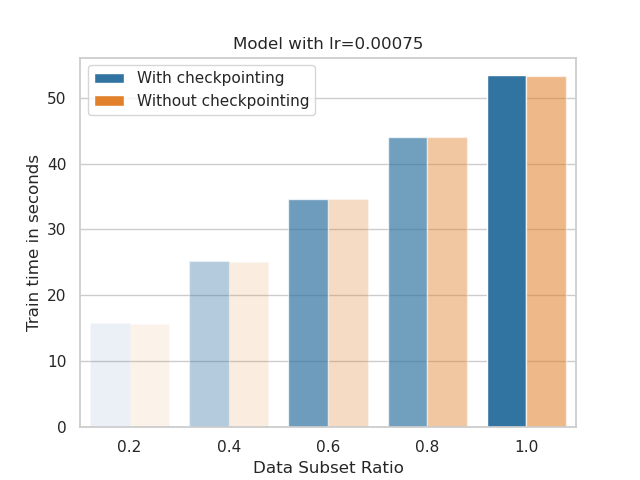
\includegraphics[width=\textwidth]{figures/22_07/2ep_smaller/train_subset_0.00075.png}
        \caption{MNIST 2 epochs, small model}
        \label{fig:9d}
    \end{subfigure}
    \caption{Visualization of the training time for every data subset ratio. A higher opacity means small validation performance difference to the optimum. An Adam optimizer and learning rate $7.5e^{-4}$ were used}
    \label{fig:9}
\end{figure}
\newpage
\begin{figure}[h]
    \centering
    \begin{subfigure}[b]{0.24\textwidth}
        \centering
        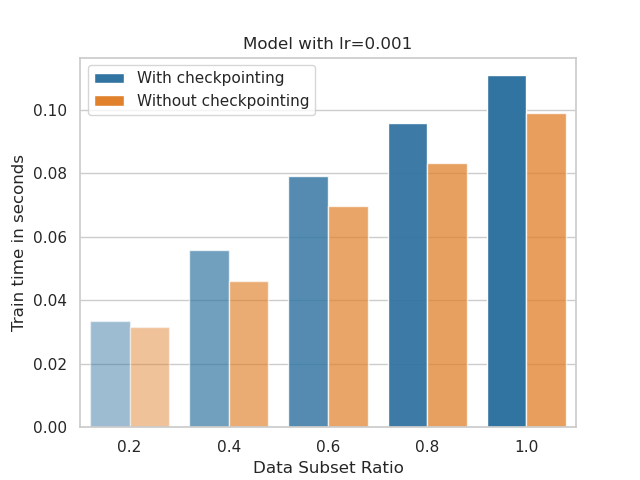
\includegraphics[width=\textwidth]{figures/22_07/iris/train_subset_0.001.png}
        \caption{IRIS}
        \label{fig:10a}
    \end{subfigure}
    %\hfill
    \begin{subfigure}[b]{0.24\textwidth}
        \centering
        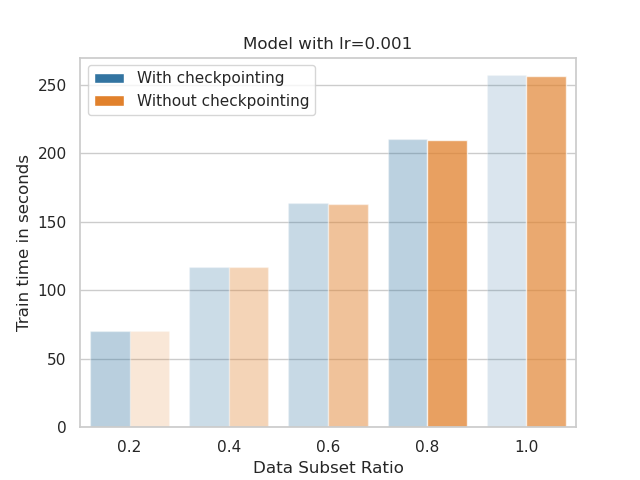
\includegraphics[width=\textwidth]{figures/22_07/10ep/train_subset_0.001.png}
        \caption{MNIST 10 epochs}
        \label{fig:10b}
    \end{subfigure}
    %\hfill
    \begin{subfigure}[b]{0.24\textwidth}
        \centering
        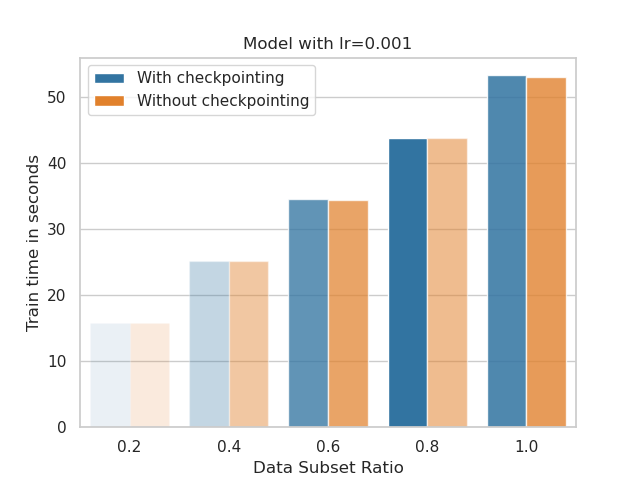
\includegraphics[width=\textwidth]{figures/22_07/2ep/train_subset_0.001.png}
        \caption{MNIST 2 epochs}
        \label{fig:10c}
    \end{subfigure}
    %\hfill
    \begin{subfigure}[b]{0.24\textwidth}
        \centering
        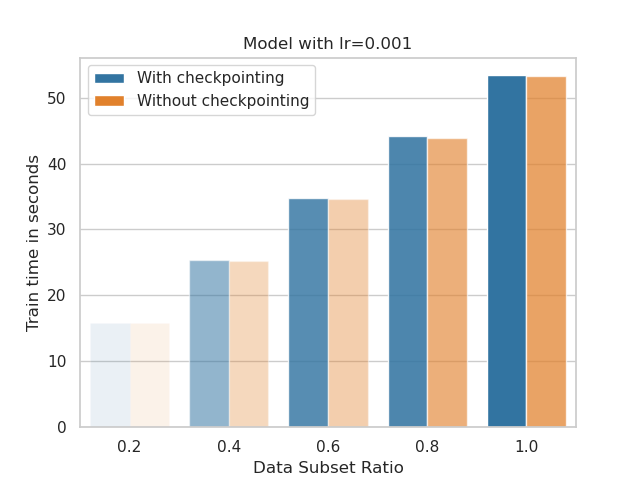
\includegraphics[width=\textwidth]{figures/22_07/2ep_smaller/train_subset_0.001.png}
        \caption{MNIST 2 epochs, small model}
        \label{fig:10d}
    \end{subfigure}
    \caption{Visualization of the training time for every data subset ratio. A higher opacity means small validation performance difference to the optimum. An Adam optimizer and learning rate $1e^{-3}$ were used}
    \label{fig:10}
\end{figure}

\begin{figure}[h]
    \centering
    \begin{subfigure}[b]{0.24\textwidth}
        \centering
        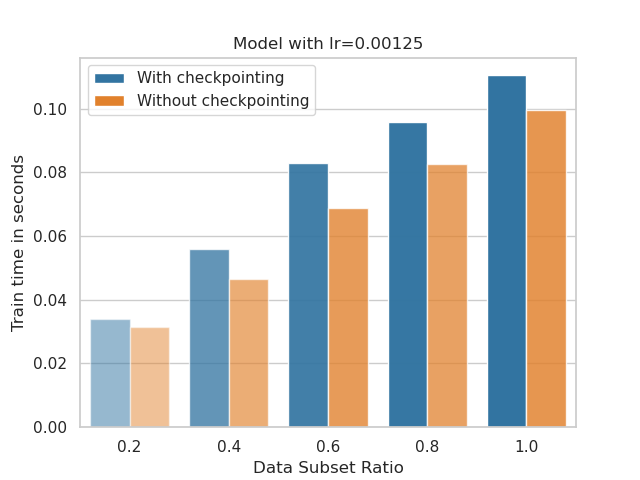
\includegraphics[width=\textwidth]{figures/22_07/iris/train_subset_0.00125.png}
        \caption{IRIS}
        \label{fig:11a}
    \end{subfigure}
    %\hfill
    \begin{subfigure}[b]{0.24\textwidth}
        \centering
        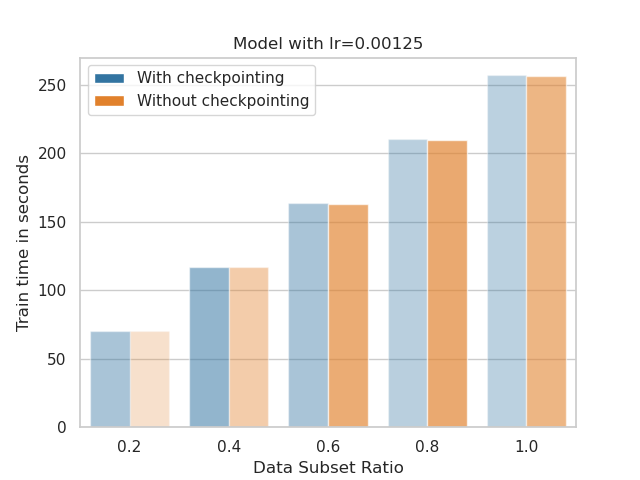
\includegraphics[width=\textwidth]{figures/22_07/10ep/train_subset_0.00125.png}
        \caption{MNIST 10 epochs}
        \label{fig:11b}
    \end{subfigure}
    %\hfill
    \begin{subfigure}[b]{0.24\textwidth}
        \centering
        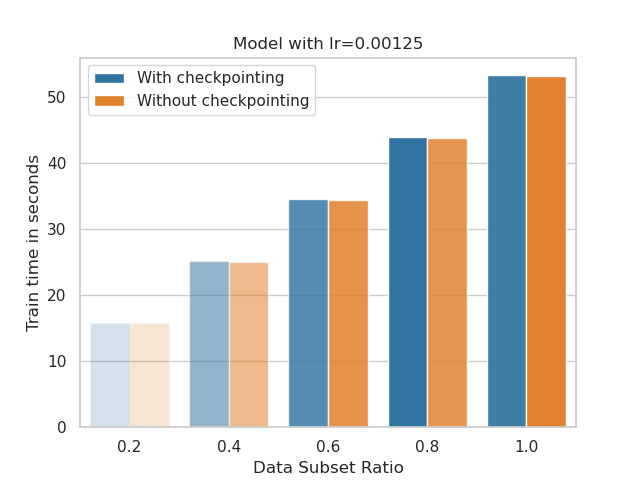
\includegraphics[width=\textwidth]{figures/22_07/2ep/train_subset_0.00125.png}
        \caption{MNIST 2 epochs}
        \label{fig:1111111111111111111111c}
    \end{subfigure}
    %\hfill
    \begin{subfigure}[b]{0.24\textwidth}
        \centering
        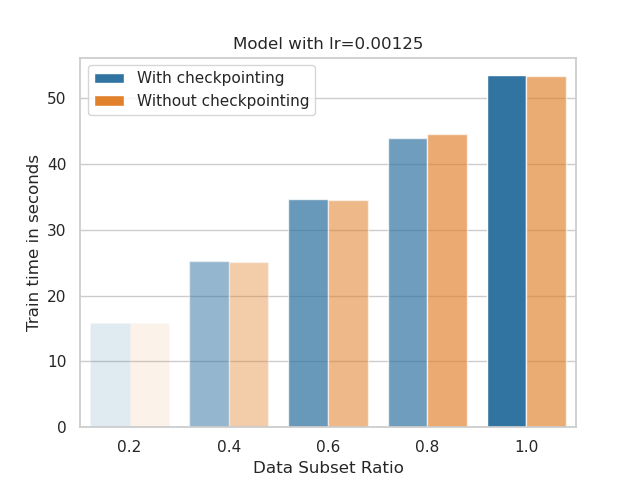
\includegraphics[width=\textwidth]{figures/22_07/2ep_smaller/train_subset_0.00125.png}
        \caption{MNIST 2 epochs, small model}
        \label{fig:11d}
    \end{subfigure}
    \caption{Visualization of the training time for every data subset ratio. A higher opacity means small validation performance difference to the optimum. An Adam optimizer and learning rate $1.25e^{-3}$ were used}
    \label{fig:11}
\end{figure}
\end{document}
